\chapter{METODOLOGIA}

%Metodologia da bibliografia
\section{Metodologia usada no Levantamento Bibliográfico}


Para atingir os objetivos que orientam este estudo, os procedimentos metodológicos foram idealizados com base em programas educacionais que visam a promoção do empreendedorismo e comportamento empreendedor em cursos de graduação, em instituições de ensino públicas e particulares, como também Startups de natureza educacional.


A metodologia de pesquisa utilizada encontra-se esquematizada na Figura \ref{figura_29}. Buscando construir um levantamento bibliográfico sólido sobre os conteúdos pretendidos neste estudo, foi realizada uma revisão sistemática utilizando como ferramenta o StArt \cite{lapes_start_2016}. A ferramenta StArt foi desenvolvida para apoiar todo processo de Revisão Bibliográfica, por meio de uma árvore hierárquica, categorizando os artigos em proximidade e níveis de aderência às palavras-chave \cite{hernandes_avaliacao_2010}.


\begin{figure}[H]
\centering
\caption{\textbf{Planejamento da pesquisa e construção do referencial teórico}}
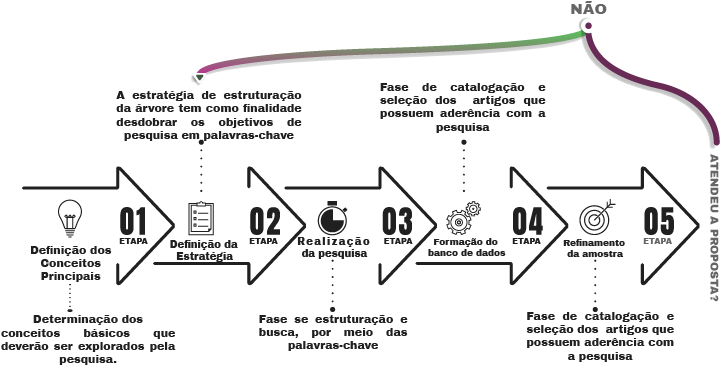
\includegraphics[scale=0.6]{Imagens/fases_pesquisa_bibliografica.png}
\fonte{Adaptado de \citeonline{fao_panorama_2017}}
\label{figura_referencial}
\end{figure}

\section{Metodologia usada no Levantamento dados sobre Transferências}

Os dados sobre transferência de tecnologias desenvolvidas pelos órgãos públicos direcionadas ao setor agrícola foram selecionados a partir das publicações disponíveis no Diário Oficial da Únião DOU.

Para delimitar o ambiente de estudo, foram adotados como indicadores os termos “Transferência de tecnologia*” e “Agricultura/Agrícola”. 

Como linha temporal foram selecionados os comentários realizados de 2016 a 2020. Dos órgãos previamente pesquisados  constam: Universidades públicas, Centros de Pesquisa e Empresas públicas.

Objetivando preservar a identidade das empresas envolvidas neste estudo, estas serão descritas como: (UP) Universidade Pública, (CP) Centro de Pesquisa, (EP) Empresa pública.
Nesta fase do  estudo, será configurada, para a coleta automatizada, a raspagem web Octoparse (versão 7.1.2, Octopus Data Inc., Walnut, CA, USA). Este software é um sistema de Eletronic Data Scraping que permite a raspagem dos dados presentes em sites abertos. 

O software foi programado para extrair os comentários sobre a percepção da estadia, desta forma, o processo de extração foi realizado em cinco passos, a saber: acesso ao site de ofertas; paginação dos locais de hospedagem; loop de raspagem dos itens; extração dos dados e abertura de novas páginas. Este processo está descrito na Figura \ref{figura_raspagem}. Durante a coleta dos dados, as publicações que se mostraram em duplicidade foram suprimidos. 



\begin{figure}[H]
\centering
\caption{\textbf{Espaço de trabalho para raspagem de publicações no Diário Oficial da União sobre transferência de tecnologia agrícola.
}}
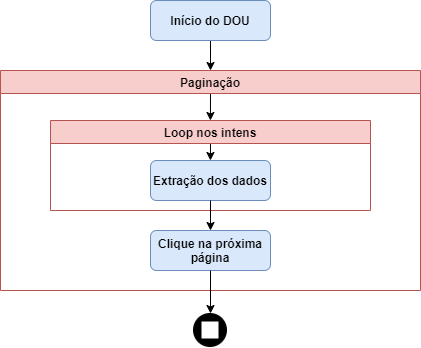
\includegraphics[scale=0.6]{Imagens/raspagem.png}
\fonte{Os Autores 2020.}
\label{figura_raspagem}
\end{figure}


\section{Desenvolvimento da matriz}









